\documentclass{article}

% if you need to pass options to natbib, use, e.g.:
%     \PassOptionsToPackage{numbers, compress}{natbib}
% before loading neurips_2019

% ready for submission
% \usepackage{neurips_2019}

% to compile a preprint version, e.g., for submission to arXiv, add add the
% [preprint] option:
%     \usepackage[preprint]{neurips_2019}

% to compile a camera-ready version, add the [final] option, e.g.:
\usepackage[]{neurips_2019}

% to avoid loading the natbib package, add option nonatbib:
%     \usepackage[nonatbib]{neurips_2019}

\usepackage[utf8]{inputenc} % allow utf-8 input
\usepackage[T1]{fontenc}    % use 8-bit T1 fonts
\usepackage{hyperref}       % hyperlinks
\usepackage{url}            % simple URL typesetting
\usepackage{booktabs}       % professional-quality tables
\usepackage{amsfonts}       % blackboard math symbols
\usepackage{nicefrac}       % compact symbols for 1/2, etc.
\usepackage{microtype}      % microtypography
\usepackage{tabularx,graphicx}

\title{Reproducing ``Towards Interpretable Reinforcement Learning Using
Attention Augmented Agents''}

% The \author macro works with any number of authors. There are two commands
% used to separate the names and addresses of multiple authors: \And and \AND.
%
% Using \And between authors leaves it to LaTeX to determine where to break the
% lines. Using \AND forces a line break at that point. So, if LaTeX puts 3 of 4
% authors names on the first line, and the last on the second line, try using
% \AND instead of \And before the third author name.

\author{%
  David S.~Hippocampus\thanks{Use footnote for providing further information
    about author (webpage, alternative address)---\emph{not} for acknowledging
    funding agencies.} \\
  Department of Computer Science\\
  Cranberry-Lemon University\\
  Pittsburgh, PA 15213 \\
  \texttt{hippo@cs.cranberry-lemon.edu} \\
  % examples of more authors
  % \And
  % Coauthor \\
  % Affiliation \\
  % Address \\
  % \texttt{email} \\
  % \AND
  % Coauthor \\
  % Affiliation \\
  % Address \\
  % \texttt{email} \\
  % \And
  % Coauthor \\
  % Affiliation \\
  % Address \\
  % \texttt{email} \\
  % \And
  % Coauthor \\
  % Affiliation \\
  % Address \\
  % \texttt{email} \\
}

\begin{document}

\maketitle

\begin{abstract}
    We attempt to reproduce Mott et al. \cite{mott2019towards} which is a recent work which introduces an attention mechanism for both 1) demonstrating what reinforcement learning agent's attend when playing Atari games, while 2) also constraining the model's representations. Our reproduction achieves moderate success.
\end{abstract}

\section{Introduction}
Various reinforcement learning methods (DQN, A3C, cite) have been used to play Atari (cite), and other similar games (DeepMindLab, cite), to great success. Largely, these methods are based on Q-learning and function approximation, relying heavily on distributed frameworks. That being said, the learned policies have remained opaque. Mott et al. begins to alleviate this nominal fog-of-war by introducing a model that admits introspection via attention mechanisms.

\section{Results}
We focus on the qualitative results of the original authors' work, aiming to find if the proposed model is able to play Atari games successfully, and if it uses attention to focus on important game elements.

\section{Architecture Overview}
Here we provide a brief overview of the architecture for the reader, and point both to the original work \cite{espeholt2018impala} and our source code \footnote{\url{https://github.com/cjlovering/torchbeast.git
}} for more details. See Fig. \ref{fig:arch} for a diagram.

\begin{figure}[ht!]
    \centering
    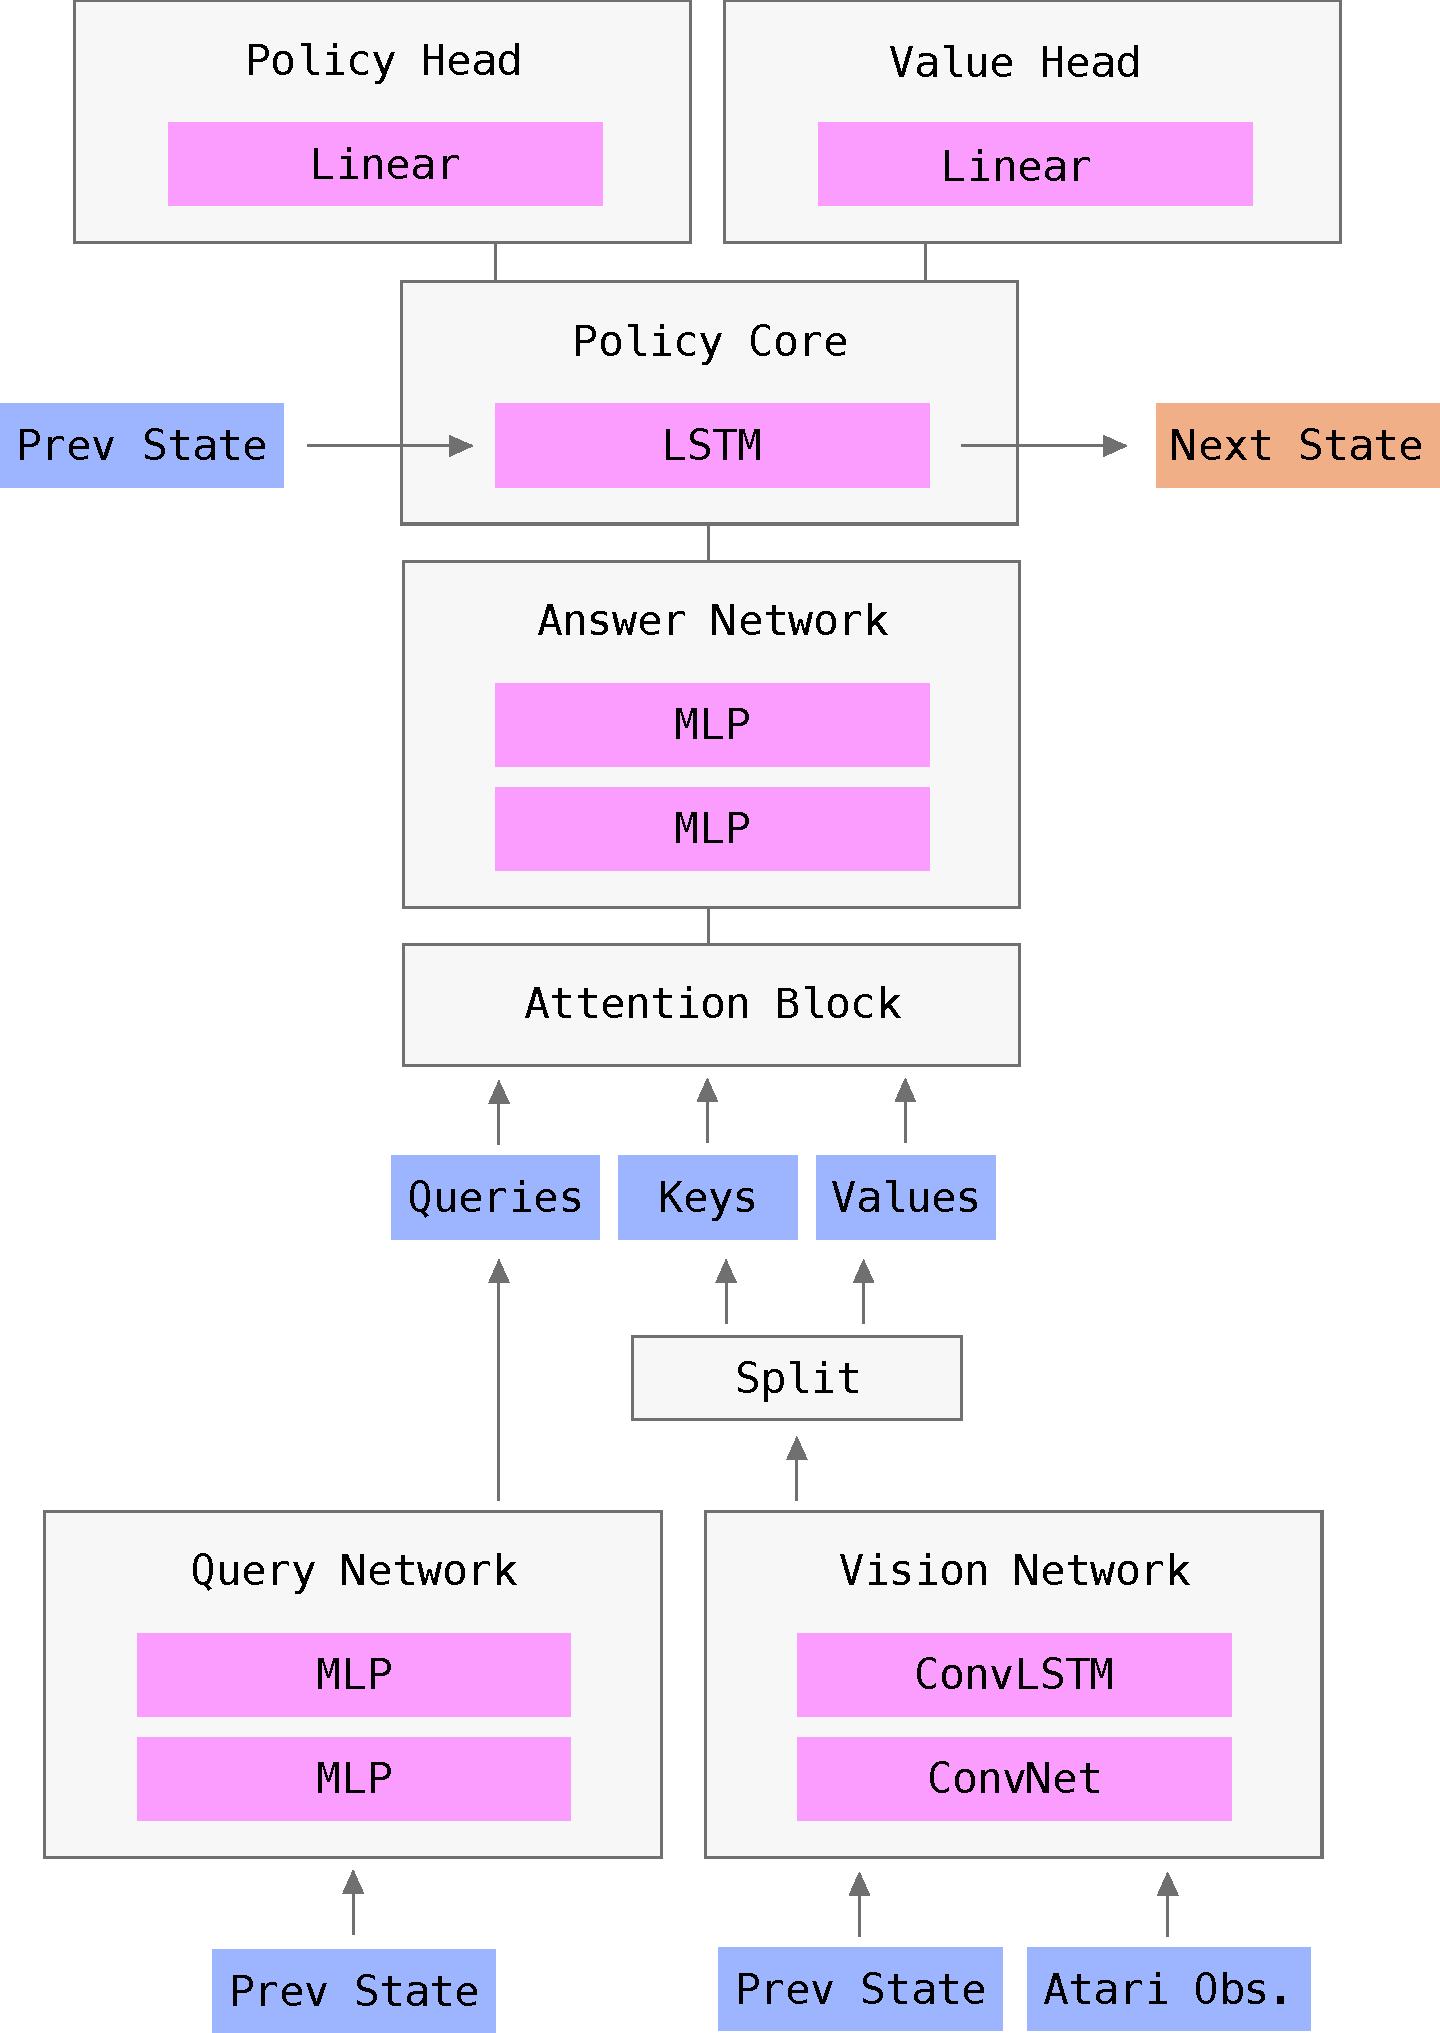
\includegraphics[width=.35\linewidth]{arch}
    \caption{Simplified architecture.}
    \label{fig:arch}
\end{figure}

\section{Implementation Details}
\subsection{Model}

We implement the proposed model as described in PyTorch\footnote{\url{https://pytorch.org/docs/master/torch.html}}, as opposed to TensorFlow\footnote{\url{https://www.tensorflow.org/}}, to validate that the architecture is platform independent. 

Due to technical limitations, our model does not feed the previous action into the next state in the central recurrent module.

\subsection{Framework}
The authors used IMPALA \cite{espeholt2018impala}, a TensorFlow-based model-training distributed system, to train their models.  IMPALA is a successor of the Asynchronous Actor Critic Advantage (A3C) \cite{}: it consists of a set of actor threads which generate offline experience trajectories, which are then dynamically batched and processed by a learner thread. The learner processes the trajectories, then updates both   its weights and the actors' weights. We use a recent PyTorch reimplementation of IMPALA called Torchbeast \cite{kuttler2019torchbeast}.

\section{Conclusions}

\subsubsection*{Acknowledgments}

Use unnumbered third level headings for the acknowledgments. All acknowledgments
go at the end of the paper. Do not include acknowledgments in the anonymized
submission, only in the final paper.

\small

\bibliography{main}
\bibliographystyle{plain}

\end{document}
